


In this use case,
We use individual reference manifest and integrity database for each target platform.
Thus, the reference manifest and integrity database are created by collector running at the target platform.
Fig \ref{fig:openpts-selfupdate} shows the operation flow of OpenPTS.


%\begin{figure}[b!p]
%  \begin{center}
%    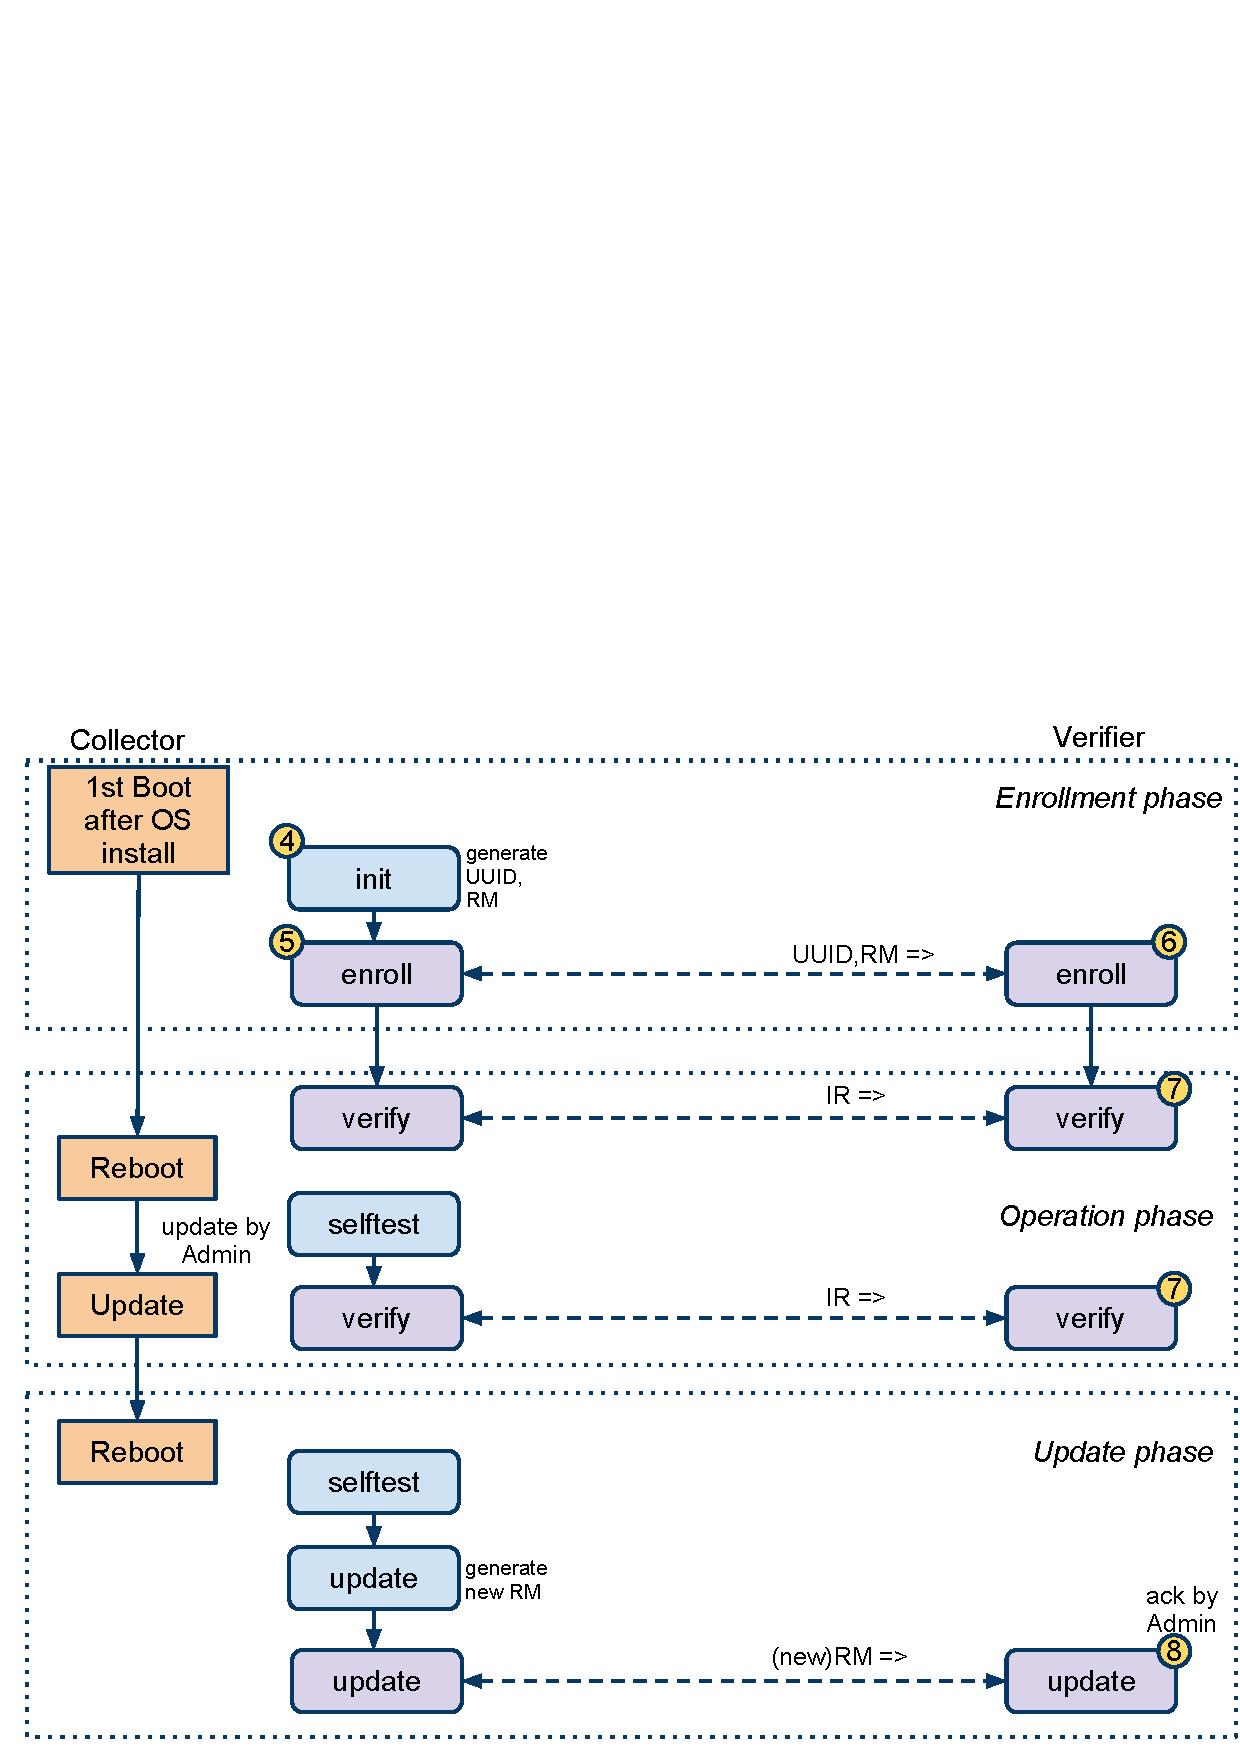
\includegraphics[width=15cm]{OpenPTS-fig-selfupdate.png}
%  \end{center}
%  \caption{TNC mode}
%  \label{fig:openptstnc}
%\end{figure}

% png - NG on Fedora 12
% pdf to eps
% yum install xpdf  - NG :-(
% pdftoeps -eps OpenPTS-fig-selfupdate.pdf -NG :-(
% yum install poppler-utils
% pdftops -eps OpenPTS-fig-selfupdate.pdf

\begin{figure}[hb!p]
  \begin{center}
    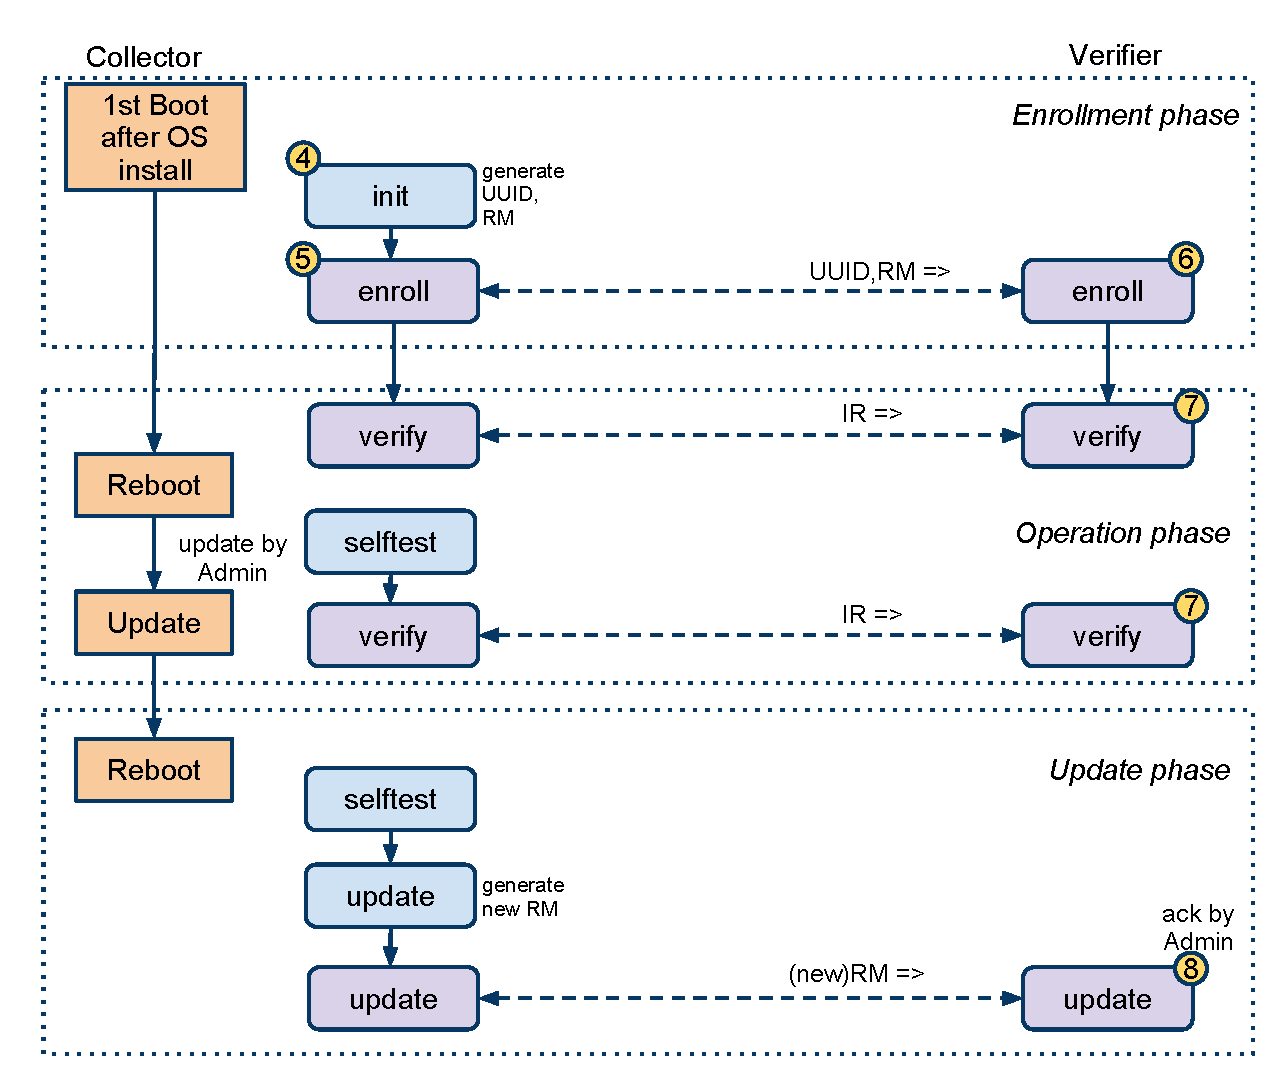
\includegraphics[width=15cm]{OpenPTS-fig-selfupdate.eps}
  \end{center}
  \caption{OpenPTS - Operation Flow}
  \label{fig:openpts-selfupdate}
\end{figure}


This use case have three operation phases as follows.

\begin{description}
\item[Enrollment phase]
We trust an installation process\footnote{If we have the EK credential of TPM, we can trust the remote platform}.
The collector generate the new UUID to identify the target and reference manifest based on the measurement of initial boot.
Thus, the reference manifests are based on actual BIOS
\footnote{OpenPTS generate manifest of actual measurement since there are no PC and BIOS vendors which disclose integrity information.}
and Operating System measurement at this phase. Verifier get the UUID and manifests from the Collector and securely stored them.

\item[Operation phase]
Verifier validate the target (remote attestation).

\item[Update phase]
After the BIOS or OS update, manifest must be updated.
The OpenPTS collector do selftest at the startup run (ptsc -s).
If validation was failed due to the change, it generates the new manifest.

If the update was expected, Verifier update the manifest too.

\end{description}

\begin{description}
 \item[Enrollment]  Initial setup (Trusted environment)
 \item[Operation]   Status check by Remote Attestation (Untrusted environment)
 \item[Update]      Update the SW status (Trusted environment)
\end{description}

\subsection{Setup the Collector (target platform)}

\subsubsection{Take the TPM ownerdhip}

Take ownership of your TPM with well known secret.

\begin{lstlisting}[style=console] 
# tpm_takeownership -y -z
\end{lstlisting}

\subsubsection{Install openpts}

(see the section 7, how to build) \\
\begin{lstlisting}[style=console]
# rpm -ivh openpts-0.2.4-1.x86_64.rpm
\end{lstlisting}

\subsubsection{Configure ptsc}

After the installation, adjust the configuration file '/etc/ptsc.conf'
If you are using GRUB-IMA, assign the validation models to PCR[4,5,8].
\begin{lstlisting}[style=source_code]
rm.num=2
rm.model.1.pcr.4=grub_pcr4hdd.uml
rm.model.1.pcr.5=grub_pcr5.uml
rm.model.1.pcr.8=grub_pcr8.uml
\end{lstlisting}
If you enabled Linux-IMA, assign the validation model of IMA to PCR[10].
\begin{lstlisting}[style=source_code]
rm.model.1.pcr.10=f12_ima_pcr10.uml
\end{lstlisting}
Set the platform infomation. e.g.
\begin{lstlisting}[style=source_code]
platform.system.manufacturer=LENOVO
platform.system.productname=745749J
platform.system.version=ThinkPad X200
platform.bios.version=6DET58WW
\end{lstlisting}
The platform infomation stored in SMBIOS can be checked by 'dmidecode' command.

\subsubsection{Setup the AIDE database (OPTIONAL)}
Create the sample AIDE DB from current IML.
(It takes long time).
\begin{lstlisting}[style=console] 
# iml2aide -c /etc/ptsc.conf -o /var/lib/aide/aide.db.gz
\end{lstlisting}
Or create the AIDE DB.
(It takes long time too).
\begin{lstlisting}[style=console]
# cp /usr/share/openpts/aide.conf  /etc/aide.conf
# aide -i
\end{lstlisting}

\subsubsection{Initialize Collector ptsc}

e.g.
\begin{lstlisting}[style=console]
 # /usr/sbin/ptsc -i
 Generate uuid               : 186bebba-2781-11e0-bcdb-001f160c9c28 
 Sign key  location          : SYSTEM
 Generate UUID (for RM)      : 19566e16-2780-11e0-bf2e-001f160c9c28 
 level 0 Reference Manifest  : /var/lib/openpts//19566e16-...9c28/rm0.xml
 level 1 Reference Manifest  : /var/lib/openpts//19566e16-...9c28/rm1.xml
\end{lstlisting}

Selftest the target platform.
\begin{lstlisting}[style=console]
 # /usr/sbin/ptsc -t
 selftest - OK
\end{lstlisting}

\subsubsection{Startup ptsc}
\begin{lstlisting}[style=console]
 # service ptsc start
 Starting ptsc:                                            [  OK  ]
\end{lstlisting}

Also, set whether ptsc should run on startup.

\begin{lstlisting}[style=console]
 # chkconfig --add ptsc
\end{lstlisting}

%\end{description}


Setup of the PTS collector is done.


\subsection{Setup the Verifier} 

Install openpts to the localhost (or any remote verifier box).

\subsubsection{Install openpts}

Use the same package, it contains both collector and verifier.

\begin{lstlisting}[style=console]
 # rpm -ivh openpts-0.2.4-1.x86_64.rpm
\end{lstlisting}


\subsubsection{Setup SSH pub-key authentication}

You have to setup SSH public key authentication between collector and verifier.
The following example uses foo@localhost as the target (collector).
e.g.
\begin{lstlisting}[style=console]
 $ ssh-keygen -t rsa
 $ ssh-copy-id foo@localhost
\end{lstlisting}


\subsubsection{Enrollment with Collector}

First, you enroll the collector.
e.g.
\begin{lstlisting}[style=console]
 $ openpts -i localhost
 /usr/bin/openpts -i -l foo localhost
 /home/foo/.openpts is missing. create [Y/n]:Y
 Target            : localhost
 Collector UUID    : 186bebba-2781-11e0-bcdb-001f160c9c28
 Manifest UUID     : 19566e16-2780-11e0-bf2e-001f160c9c28
 manifest[0]       : /home/foo/.openpts/186bebba-...9c28//19566e16-...9c28/rm0.xml
 manifest[1]       : /home/foo/.openpts/186bebba-...c9c28//19566e16-...c9c28/rm1.xml
 configuration     : /home/foo/.openpts/186bebba-...9c28/target.conf
 validation policy : /home/foo/.openpts/186bebba-...9c28/policy.conf
\end{lstlisting}
target.conf, policy.conf (and aide.ignore) are automaticaly generated.
rm0.xml, rm1.xml and aide.db.gz are received from collector.
To override existing setting, use "-f" option.
\begin{lstlisting}[style=console]
 $ openpts -i -f localhost
\end{lstlisting}
See the Table \ref{table:openpts:file} about the file used by openpts command.

%\end{description}
%
%\subsection{Remote Attatation (localhost)} 
%\begin{description}
\subsubsection{Remote Attestation}

\begin{lstlisting}[style=console]
 $ openpts -v localhost
 Target         : localhost
 Collector UUID : 186bebba-2781-11e0-bcdb-001f160c9c28
 Manifest UUID  : 19566e16-2780-11e0-bf2e-001f160c9c28
 username(ssh)  : default
 port(ssh)      : default
 policy file    : /home/foo/.openpts/186bebba-...9c28/policy.conf
 property file  : /home/foo/.openpts/186bebba-...9c28/vr.properties
 integrity      : valid
\end{lstlisting}

%\end{description}


\subsection{Collector update the manifests} 


At the startup, the collector selftest the platform.
If the seftest was faild, the collector generate the new manifest against current measurements.
This happen if you update any relevent components, such as the BIOS or OS image.

\subsection{Verifier update the manifests} 

\subsubsection{Accept the change happen on the collector}

When the collector update the manifest, 
verification of the target was fail since there are mismatch between the collector and the verifier.
\begin{lstlisting}[style=console]
 $ openpts -v localhost
 Target         : localhost
 Collector UUID : 1dbac28e-2787-11e0-b84a-001f160c9c28
 Manifest UUID  : 1df210fe-2787-11e0-b84a-001f160c9c28
 port           : 6678 (localhost)
 policy file    : /home/foo/.openpts/1dbac28e-2787-11e0-b84a-001f160c9c28/policy.conf
 property file  : /home/foo/.openpts/1dbac28e-2787-11e0-b84a-001f160c9c28/vr.properties
 integrity      : unknown (INTERNAL ERROR) rc=35
 Reasons
     0 Missing Reference Manifest(RM)
     1 Collector hostname = localhost
     2 Collector UUID = 1dbac28e-2787-11e0-b84a-001f160c9c28
     3 Collector RM UUID = 33b88c38-2787-11e0-adc0-001f160c9c28
 New reference manifest exist. if this is expected change, update the manifest by openpts -i -f 
\end{lstlisting}
If this is predicted or legitimate change. Update the target information.
\begin{lstlisting}[style=console]
 $ openpts -i -f  localhost
 Target            : localhost
 Collector UUID    : 1dbac28e-2787-11e0-b84a-001f160c9c28
 Manifest UUID     : 33b88c38-2787-11e0-adc0-001f160c9c28
 manifest[0]       : /home/foo/.openpts/1dbac28e-...c9c28//33b88c38-...9c28/rm0.xml
 manifest[1]       : /home/foo/.openpts/1dbac28e-...9c28//33b88c38-...9c28/rm1.xml
 configuration     : /home/foo/.openpts/1dbac28e-...9c28/target.conf
 validation policy : /home/foo/.openpts/1dbac28e-...9c28/policy.conf
\end{lstlisting}
Then verify again.
\begin{lstlisting}[style=console]
 $ openpts -v localhost
 Target         : localhost
 Collector UUID : 1dbac28e-2787-11e0-b84a-001f160c9c28
 Manifest UUID  : 33b88c38-2787-11e0-adc0-001f160c9c28
 username(ssh)  : default
 port(ssh)      : default
 policy file    : /home/foo/.openpts/1dbac28e-...9c28/policy.conf
 property file  : /home/foo/.openpts/1dbac28e-...9c28/vr.properties
 integrity      : valid
\end{lstlisting}


\subsection{Check the status}

\subsubsection{Status of the collector}

\begin{lstlisting}[style=console]
# /usr/sbin/ptsc -D
openpts version 0.2.2.svn

config file                 : /etc/ptsc.conf
UUID                        : 186bebba-...c9c28 (/var/lib/openpts/uuid)
IML access mode             : TSS
  Runtime IML type          : IMA (kernel 2.6.32)
RM UUID (current)           : 19566e16-2780-11e0-bf2e-001f160c9c28
RM UUID (for next boot)     : (null)
List of RM set              : 1 RM set in config dir
                               ID  UUID                 date(UTC)         status
                              -------------------------------------------------------
                                0 d5086d88-...c9c28 2011-01-24-05:50:21 state=UNKNOWN
                              -------------------------------------------------------
Integrity Report            : /var/lib/openpts/ir.xml
Model dir                   : /usr/share/openpts/models
                              Behavior Models
                              PCR lv  FSM files
                              -----------------------------------------------------
                               0  0  /usr/share/openpts/models/bios_pcr0.uml
                               1  0  /usr/share/openpts/models/bios_pcr1.uml
                               2  0  /usr/share/openpts/models/bios_pcr2.uml
                               3  0  /usr/share/openpts/models/bios_pcr3.uml
                               4  0  /usr/share/openpts/models/bios_pcr4.uml
                               4  1  /usr/share/openpts/models/grub_pcr4hdd.uml
                               5  0  /usr/share/openpts/models/bios_pcr5.uml
                               5  1  /usr/share/openpts/models/grub_pcr5.uml
                               6  0  /usr/share/openpts/models/bios_pcr6.uml
                               7  0  /usr/share/openpts/models/bios_pcr7.uml
                               8  1  /usr/share/openpts/models/grub_pcr8.uml
                              10  1  /usr/share/openpts/models/f12_ima_pcr10.uml
                              -----------------------------------------------------
\end{lstlisting}

\subsubsection{Status of the verifier}
\begin{lstlisting}[style=console]
$ openpts -D
Show openpts config
--------------------------------------------------------------------
config file               : /home/foo/.openpts/openpts.conf
uuid                      : 240fbb66-6fdb-11e0-a735-001f160c9c28
--------------------------------------------------------------------
target[0] uuid            : cf9cfa32-6fba-11e0-84de-001f160c9c28
target[0] config          : /home/foo/.openpts/cf9cfa32-6fba-11e0-84de-001f160c9c28/target.conf
target[0] hostname        : localhost
--------------------------------------------------------------------
target[1] uuid            : 0445a354-6fdb-11e0-aa91-001f160c9c28
target[1] config          : /home/foo/.openpts/0445a354-6fdb-11e0-aa91-001f160c9c28/target.conf
target[1] hostname        : host023
--------------------------------------------------------------------
\end{lstlisting}
%\end{description}

